\chapter{Clustering}  \label{clustering}
In Chapter~\ref{ch4}, I described our anti-unification algorithm to construct an anti-unifier from AUASTs of a pair of LMs with special attention to logging calls. Recall that the general point of this study is to provide a concise description of where logging calls happen in source code by constructing structural generalizations that represent the detailed commonalities and differences between AUASTs of LMs. To this end, we should develop an algorithm that:
\begin{itemize} [leftmargin=.5in]
\item clustering Java methods showing different usages of logging calls into separate clusters.
% using a measure of similarity.
%classifies AUASTs of LMs into clusters using a measure of similarity such that AUASTs in each group has maximum similarity with each other and minimum similarity to other ones.

%such that entities
\item abstracts AUASTs of LMs of each group into a structural generalization representing the commonalities and differences between them.
%abstracts structural correspondences of ASTs
\end{itemize}

Clustering is the classification of a collection of unlabelled data items into meaningful groups \cite{jain1999data}, where category labels are obtained from the similarities between data items. Therefore, before the use a clustering algorithm to classify a set of AUASTs, I need to first define a similarity metric. To develop a measure of similarity between AUASTs, I used the similarity function described in Section~\ref{meth-similarity}. To perform clustering on a set of AUASTs of LMs, I developed a modified version of an agglomerative hierarchical clustering algorithm suited to my application. The clustering algorithm is a bottom-up approach that starts with singleton clusters, each contains one AUAST, and then it repeatedly merges the closest clusters that are the ones with maximum similarity between their AUASTs. To evaluate my approach, I have implemented the clustering tool (Section~\ref{clusteringTool}) and conducted an experimental study through the application of it on the test suite introduced in Section~\ref{study1_setup}. I will describe my experimental study and discuss the results in Section~\ref{clustering-assessment}.



%However, to cluster Java methods that use logging calls, a further step should be taken that is the application of a clustering algorithm on the set of AUASTs of LMs extracted from the source code. Therefore, I have developed a modified version of an agglomerative hierarchical clustering algorithm suited to my application.
% when it is needed to merge two clusters.
%Figure~\ref{fig:meth_overview} shows an overview of the general process of our anti-unification technique, as will be described in the following sections.



\section{The hierarchical clustering algorithm} \label{clustering-alg}
%\subsection{Anti-unifying a set of AUASTs} \label{meth-clustering}
To anti-unify a set of AUASTs, I have developed a modified version of an agglomerative hierarchical clustering algorithm as described below:
%agglomerative hierarchical clustering(AHC)???

\begin{enumerate} [leftmargin=.5in]
\item Start with singleton clusters, each contains one AUAST
\item Create a similarity matrix by computing pairwise similarities between clusters
\item Find the closest clusters (a cluster pair with maximum similarity)
\item Merge the closest cluster pair and replace them with a new cluster containing the anti-unifier of AUASTs of the two clusters
\item Update the similarity matrix by computing the similarity between new cluster and all remaining clusters
\end{enumerate}
\begin{itemize} [leftmargin=.5in]
\item Repeat steps 3, 4, and 5 until the similarity between closest clusters becomes below a predetermined threshold value
\end{itemize}


The hierarchical algorithms use a similarity matrix. It employs a $n \times n$ similarity matrix for a set of $n$ AUASTs, where an element in row $i$ and column $j$ represents the similarity between the $i^{\text{th}}$ and the $j^{\text{th}}$ clusters. In this algorithm, the similarity between a pair of clusters is defined as the similarity between their AUASTs, which is computed through the algorithm described in Section~\ref{meth-similarity}. However, to prevent the combination of a cluster pair when the usage of logging is different, I adjusted the similarity between them to zero. That is, if the anti-unification of AUASTs of a cluster pair does not allow the anti-unification of log statements with each other (as the structures enclosing them are not corresponded), they should be in separate clusters. I also used the anti-unification algorithm described in Section~\ref{meth-antiUnifier} to construct structural generalizations.

%threshold????
Figure~\ref{fig:overview2} illustrates the clustering process for a sample set of 5 AUASTs using the initial similarity matrix depicted in Figure~\ref{matrix}. In the first and second iterations, clusters 1 and 2, and then clusters 4 and 5 are selected as the closest clusters, merged, and replaced by clusters 6 and 7, respectively. If threshold value is determined as $Threshold A = 0.20$, the process will be terminated as the similarity between the closest clusters, which are clusters 3 and 6 is below this threshold; otherwise, these clusters will be merged and replaced by cluster 8. However, the similarity between AUASTs of clusters 7 and 8 is zero, and thus they should not be merged with each other. In this study, the similarity threshold is determined through informal experimentation.


\begin{figure} [H]
\begin{displaymath}
    similarity = \left[
        \begin{matrix}
        1.00 &  &  &  &   \\
0.28 & 1.00 &  &  &  \\
0.12 & 0.17 & 1.0 &  &  \\
0.00 & 0.00 & 0.00 & 1.0 &  \\
0.00 & 0.00 & 0.00 & 0.21 & 1.00
        \end{matrix}   \right]
\end{displaymath}
 \caption{The similarity matrix for a sample set of 5 AUASTs.}
  \label{matrix}
\end{figure}




\begin{figure} [H]
  \centering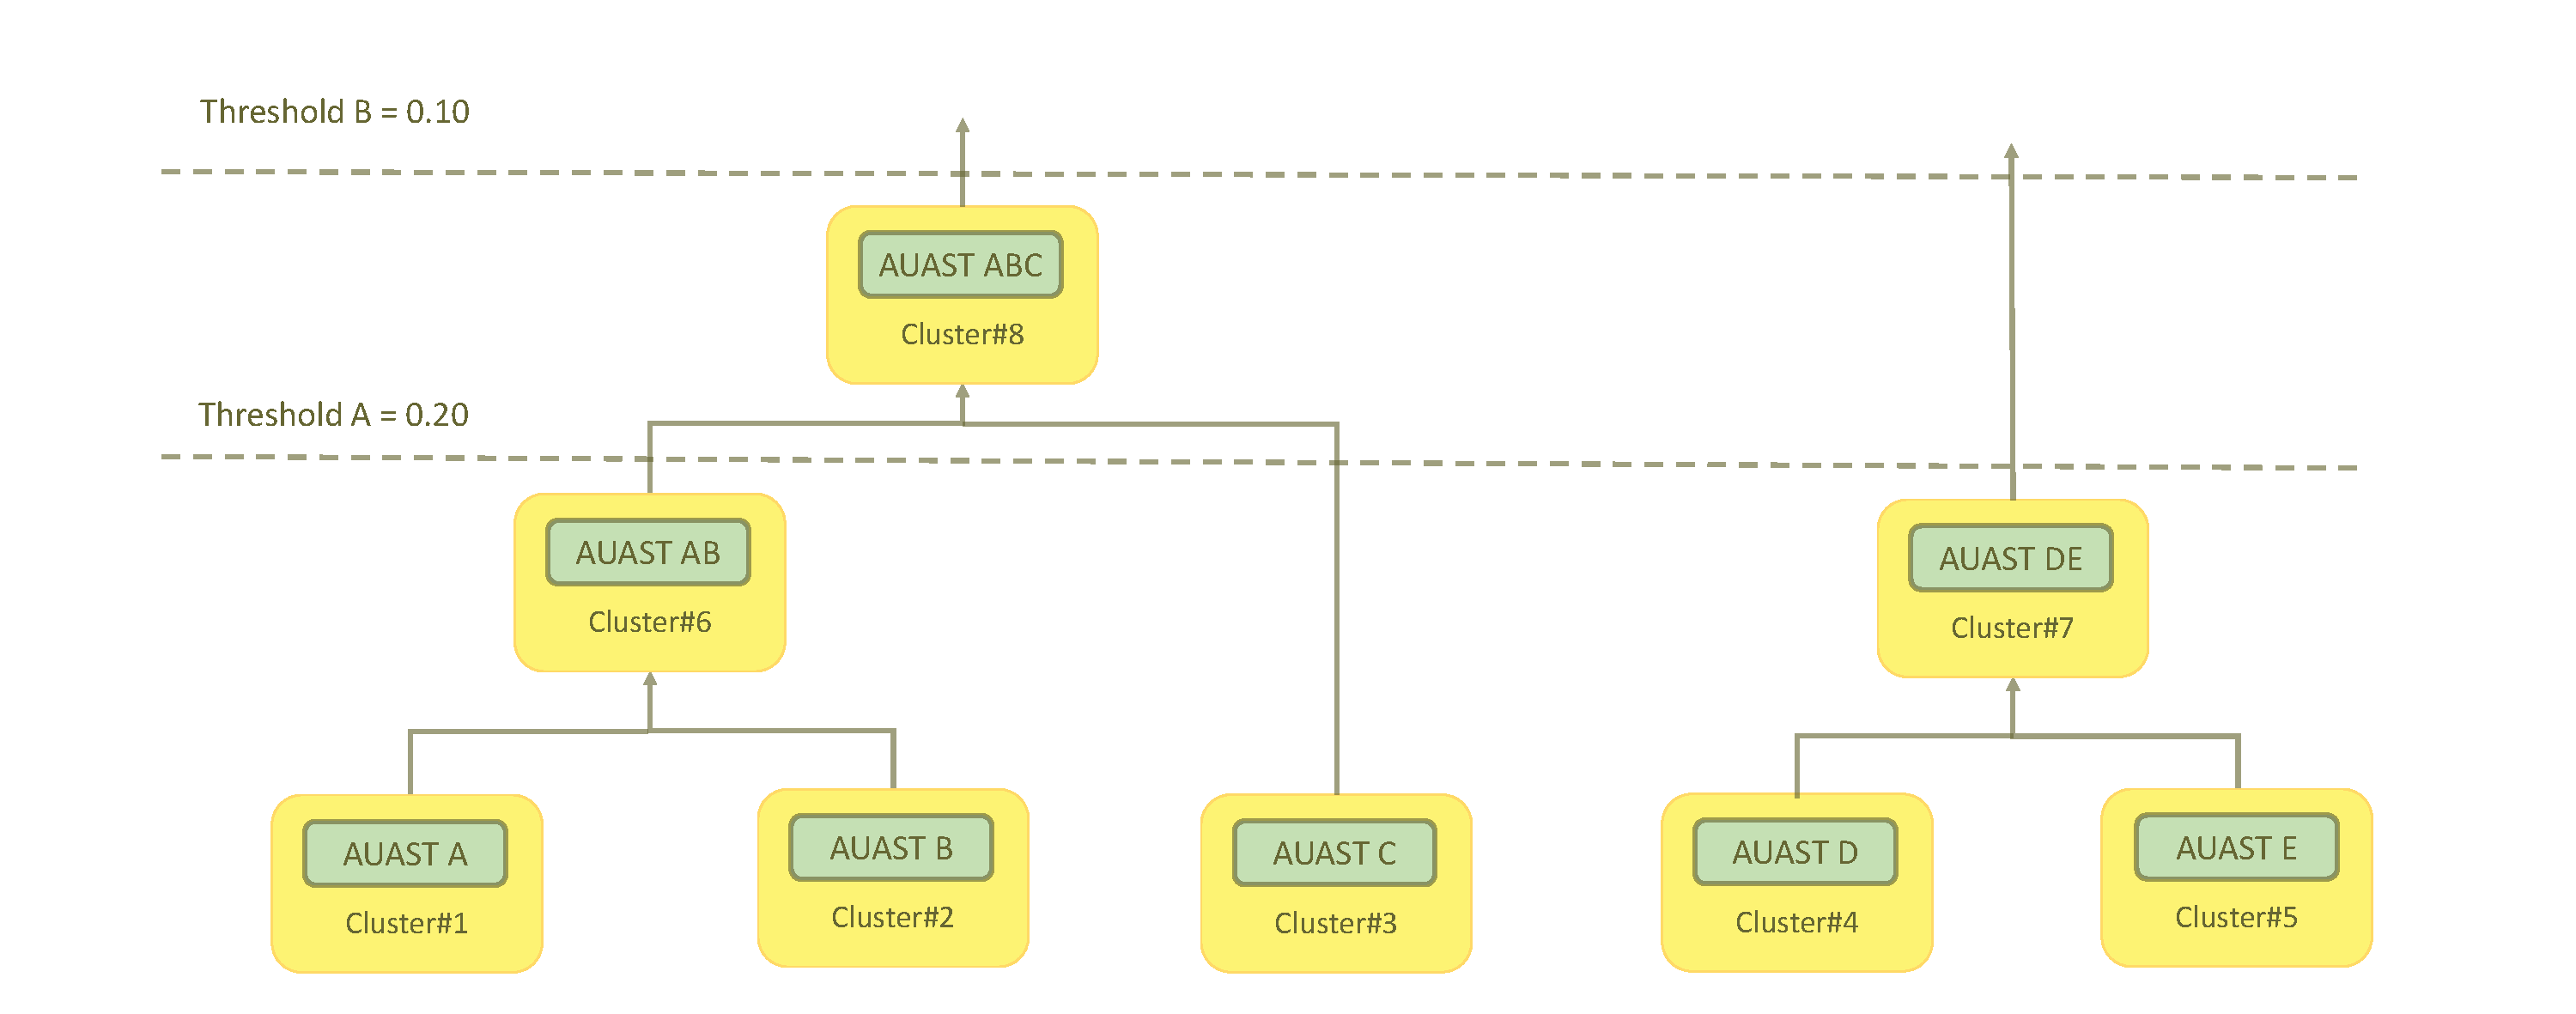
\includegraphics [width = \textwidth]{Drawing4/overview2.pdf}
  \caption{The agglomerative hierarchical clustering process on a sample set of  5 AUASTs using the initial similarity matrix shown in Figure~\ref{matrix}. The threshold value indicates the number of clusters we will come up with.}
  \label{fig:overview2}
\end{figure}


\section{Evaluaton} \label{evaluation}
To evaluate the clustering approach, I have implemented a tool, and conducted an experiment on the set of AUASTs of LMs described in Table~\ref{table:ljms}. The clustering tool is an Eclipse plug-in built atop the anti-unifier building tool that inputs a set of AUASTs of LMs extracted from the source code, applies the clustering algorithm on them, and outputs a structural generalization for each cluster.

%\section{An assessment of the Clustering tool} \label{clustering-assessment}
%To assess the effectiveness of my clustering algorithm and the tool support, I conducted an experiment on the set of AUASTs of LMs described in Table~\ref{table:ljms}.
%The tool is developed atop the anti-unifier-building tool.

\subsection{Setup}  \label{study3-setup}
I manually attempted to perform the hierarchical clustering on the set AUASTs of LMs in the test suite and constructed the detailed anti-unifier view for each cluster. Anti-unifiers were discarded when the anti-unification of LMs did not allow the anti-unification of logging calls with one another, as the Java elements enclosing them were not found to be corresponded. I also measured the level of similarity between AUASTs in each cluster by computing the ratio of common Java elements in the detailed anti-unifier view to the total number of Java elements of all AUASTs in that cluster. I also ran the clustering tool on the set of AUASTs to classify them using the similarity measurement.

\subsection{Results}  \label{study3-results}
I present the results of my analysis in Table~\ref{results_clustering}. The analysis of the output has been divided into three categories: correspondence, similarity, and separateness. The analysis of correspondence and similarity was described in Section~\ref{study2-results}. "Separateness" refers to my tools' ability to cluster Java method with different usages of logging calls into separate groups, and the ones with similar usages of logging calls into the same clusters. By similar usage of logging calls, I mean the anti-unification of AUASTs of Java methods in each cluster allows the anti-unification of their log statement nodes with one another, as well.

%the usage of logging in Java methods of each cluster is similar that they should be grouped in the same cluster, and dissimilar to the other Java methods in the other clusters that should be scattered in different clusters.
% "Relevancy" refers to the number of LMs in each cluster that are detected to berelevant as their logging calls can be anti-unified with one another and cannot be anti-unified with logging calls of LMs in the other clusters.
%AUASTs of all LMs in each cluster

\begin{figure} [H]
  \centering
  \begin{tabular}{|c|c|c|c|c|c|c|}
    \hline

    \multirow{2}{*}{Cluster}&\multicolumn{2}{c|}{Correspondence}&\multicolumn{2}{c|}{Similarity}&\multirow{2}{*}{Separateness}\\
    \cline{2-5}
    &Correct (\%)&Incorrect&human&tool&\\
    \hline
    1&28(100)&0&0.09&0.09  &\cmark \\
    \hline
    3&24(92)&2&0.19&0.2& \cmark\\
    \hline
      2&9(100)&0&0.25&0.25& \cmark\\
 	\hline
  \end{tabular}
  \caption{Results from applying the clustering tool to the test suite described in Table~\ref{table:ljms}}
  \label{results_clustering}
\end{figure}

The clustering tool succeeded in detecting the separateness amongst AUASTs of test cases correctly. Clusters 1, 2, and 3 contain logged Java methods of cases (1, 3, 5, 8), (4, 6, 7), and (2, 9, 10), respectively, as detected by my manual inspection. It also successfully calculated the similarity between LMs of 2 clusters out of 3. In Cluster 2, the error in detecting correspondences originated from the previous study and propagated to the clustering study. However, it is trivial (0.01) and would have a low impact on our final results.
%between the LMs of our test suite.

\section{Summary} \label{meth2-summary}
I have presented a modified version of the agglomerative hierarchical clustering algorithm to classify Java methods with different usages of logging calls into separate groups. This algorithm is implemented as an Eclipse plug-in that takes a set of AUASTs of LMs, clusters them via the application of the anti-unifier building tool to measure pairwise similarities between the AUASTs of cluster pairs, and generates a structural generalization for each cluster. Furthermore, an experimental study was conducted to validate the effectiveness of my clustering algorithm and the tool support on a test suite.
